\section{Lösungsvorschläge}

\subsection{Aufgabe 4.1}

s. Abbildung~\ref{fig:requirementsengineering}.


\subsection{Aufgabe 4.2}

Eine Domänenanalyse sollte durchgeführt werden, damit Hintergründe und (geschäftl.) Umfeld des Projektes und des zu erstellenden Produktes klar sind.\\
Eine Einarbeitung in fachliche Konzepte und eine Aneignung der Sprache / des Vokabulars / der Fachbegriffe erleichtert zudem die Kommunikation in den initialen und nachfolgenden Phasen des Projektes und der Projektplanung.\\
Kenntnisse über die Fachlichkeit ermöglicht es zudem, wichtige Informationen zu verstehen und sich diese für zukünftige Diskussionen und Entwürfe zu merken.

\subsection{Aufgabe 4.3}
Fachliteratur ermöglicht es, sich einen Überblick über die Grundlagen und Konzepte des Projektes und des zu erstellenden Produktes zu verschaffen.\\
Gespräche mit Kollegen können dazu beitragen, das Verständnis für bestimmte Themen zu schärfen, entweder in der Diskussion über eine bestimmte Thematik, oder - wenn der Kollege bereits
eingearbeitet ist - häufig festgestellte Unklarheiten aus dem Weg zu räumen und Mißverständnisse gegenüber bestimmter Themen zu klären.\\
Erst dann sollte im Gespräch mit dem Kunden bzw. Fachexperten über Spezifikationen oder Details gesprochen werden, damit man nicht allzu häufig aufgrund fehlendem Fachwissens später rückfragen muss.\\
Darüberhinaus kann mit einer soliden Grundlage an Fachwissen auch Funktionalität und Bedürfnisse vorhergeahnt werden, außerdem kann Funktionalität im Vorhinein berücksichtigt werden, die nur auf Basis des Fachwissens als selbstverständlich erscheint.

\subsection{Aufgabe 4.4}
s. Tabelle~\ref{tab:stakeholder}.

\subsection{Aufgabe 4.5}
\textbf{Für} die Kunden und Mitarbeiter des Straßenbahnunternehmens XYZ sowie die Kunden der DB, \\
\textbf{die} Auskünfte zu Fahrplänen, Störungen und Preisen im vom XYZ bedienten Nahverkehr benötigen,\\
\textbf{ist} die webbasierte Softwarelösung ABC eine Auskunftsplattform,\\
\textbf{die} diese Informationen über das Internet bzw. die DB bereitstellt.\\
\textbf{Anders als} mit schriftlichen Plänen oder Aushängen ist es \textbf{mit Produkt} ABC möglich, diese Informationen von überall stets aktuell beziehen zu können sowie diese Informationen anderen Systemen zur Verfügung zu stellen.\\
Dies verspricht eine höhere Nutzerzufriedenheit sowie mehr Kunden.


\subsection{Aufgabe 4.6}

s. Abbildung~\ref{fig:aufgabe4-6}.

\begin{figure}
    \centering
    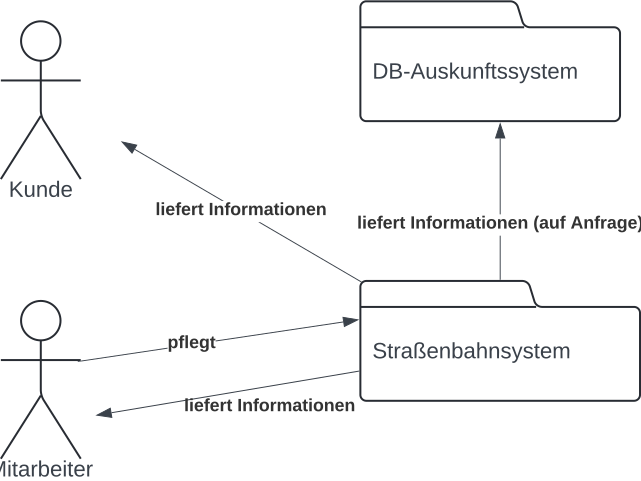
\includegraphics[scale=0.35]{chapters/Requirements Engineering/img/aufgabe4.6}
    \caption{}
    \label{fig:aufgabe4-6}
\end{figure}

